\documentclass{article}
\usepackage{ztikz}
\ztikzLoadModule{cache, gnuplot}
\usepackage{pgfplots}
\usepgfplotslibrary{polar}


\begin{document}
\centering
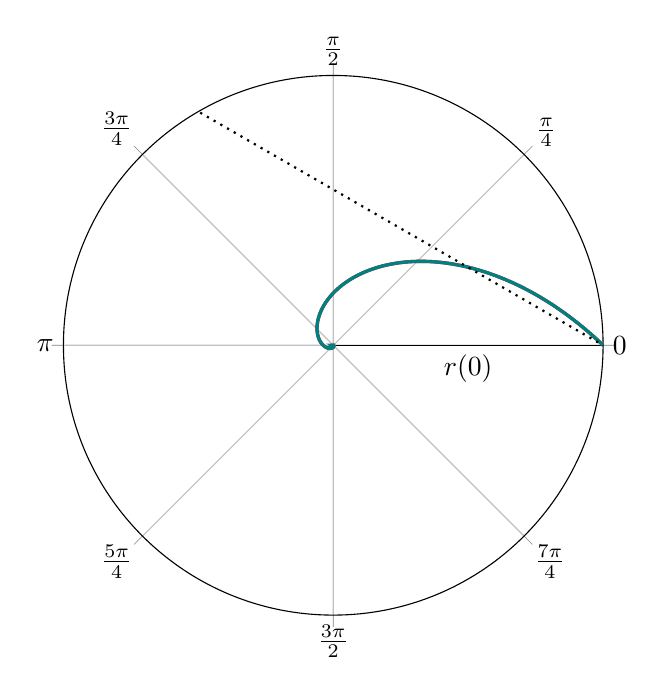
\begin{tikzpicture}
    \begin{polaraxis} [
        xtick={0, 45, 90, 135, 180, 225, 270, 315}, 
        xticklabels={0, $\frac{\pi}{4}$, $\frac{\pi}{2}$, $\frac{3\pi}{4}$, $\pi$, $\frac{5\pi}{4}$, $\frac{3\pi}{2}$, $\frac{7\pi}{4}$},
        ymax=1,
        ylabel=$r(0)$,
        y label style={anchor=north},
        minor y tick num=0,
        ytick=\empty
    ]
    \addplot [domain=0:720, samples=720, red, very thick] {e^(-x*tan(pi/3))};
    \addplot [domain=0:720, samples=720, teal, very thick] {exp(-x*tan(pi/3))};
    \addplot [domain=-4:4, samples=100, black, thick, dotted, data cs=cart] {-x/sqrt(3) + 1/sqrt(3)};
    \end{polaraxis}
    % my code
    \begin{scope}[scale=5]
      \PolarPlot[0:2*pi][red]{exp(-t*tan(pi/3))}
      \Plot[-0.5:1.5][teal]{-1/sqrt(3)*x + 1/sqrt(3)}
    \end{scope}
\end{tikzpicture}
\end{document}
